\documentclass[xcolor=pdftex,dvipsnames,table]{beamer}
\usepackage{subfigure}
\usepackage{amsbsy}
\usepackage{tikz}
\usetikzlibrary{arrows}
\usepackage{amsmath,graphicx,dsfont,color}
\usepackage{amsfonts}
\usepackage{amssymb}
\usepackage{array}

\bibliographystyle{apalike}

\setbeamertemplate{bibliography item}{\insertbiblabel}
\setbeamertemplate{bibliography entry title}{}
\setbeamertemplate{bibliography entry location}{}
\setbeamertemplate{bibliography entry note}{}

%Definitiona

\newcommand{\x}{\mathbf{x}}
\newcommand{\X}{\mathbf{X}}
\newcommand{\W}{\mathbf{W}} %Weight
\newcommand{\bais}{\mathbf{b}}%Bais
\newcommand{\act}{\texttt{g}}%Activation
\newcommand{\loss}{L}
\newcommand{\pdata}{\hat{p}_{\texttt{data}}}
\newcommand{\nsize}{n}
\newcommand{\param}{\boldsymbol{\theta}}
\newcommand{\featmap}{\boldsymbol{\phi}}
\newcommand{\EV}{\mathbb{E}}









\title{Deep Learning for Image Analysis - Introduction}
\author{Thomas Walter, PhD}
\date{Centre for Computational Biology (CBIO) \\
	  MINES Paris-Tech, PSL Research University \\
	  Institut Curie, PSL Research University \\
	  INSERM U900}

%1) MINES ParisTech, PSL Research University, CBIO-Centre for Computational Biology, F-75006 Paris, France 
%2) Institut Curie, PSL Research University, F-75005 Paris, France
%3) INSERM, U900, F-75005 Paris, France


%To include LOGO?
%\logo{\includegraphics[width=.1\columnwidth]{MinesLogo}}
\useinnertheme{rounded}
\usecolortheme{rose}

\usepackage{xcolor}
\definecolor{lightblue}{RGB}{0,200,255}

\setbeamertemplate{footline}[frame number]{}
\setbeamertemplate{navigation symbols}{}
\setbeamertemplate{section in toc}[square]
%\setbeamercolor{section number projected}{bg=lightblue}


\begin{document}


\begin{frame}
\titlepage
\end{frame}

\begin{frame}{Overview}
\tableofcontents
\end{frame}

%%%%%%%%%%%%%%%%%%%%%%%%%%%%%%%%%%%%%%%%%%%%%%%%%%%%%%%%%%%%%%%%%%%%%%%%%
%%%%%%%%%%%%%%%%%%%%%%%%%%%%%%%%%%%%%%%%%%%%%%%%%%%%%%%%%%%%%%%%%%%%%%%%%
\section{Introduction: Artificial Intelligence and Machine Learning}
\frame{\tableofcontents[currentsection]}

\begin{frame}{Definition of Artificial Intelligence}
%\begin{definition}
%	Artificial intelligence (AI) is intelligence demonstrated by machines, in contrast to the natural intelligence displayed by humans and other animals.
%\end{definition}
\begin{itemize}
	\item The definition of the term "intelligence" is highly controversial. Usually, one understands by intelligence the capacity of an individual to reason logically, to understand complexity, to learn more or less abstract concepts, to plan and to solve problems in varying conditions. 	
	\item Artificial intelligence (AI) is intelligence demonstrated by machines, in contrast to the natural intelligence displayed by humans and other animals. 
	\item In 1956, AI became a field of research. AI can be broken down into many subfields: knowledge representation, planning, natural language processing, object manipulation (robotics), $\ldots$
\end{itemize}
\end{frame}

\begin{frame}{Definition of Machine Learning}
\begin{itemize}
	\item Machine Learning is concerned with the technology that enables computer programs to improve their performance at a certain task by experience. 
	\item In \textbf{supervised learning}, this experience comes in form of a \textbf{training set} of annotated samples, i.e. a set of observations $x_i$ together with their annotation $y_i$.
	\item In \textbf{unsupervised learning}, there are no annotations, i.e. no value of $y_i$ is given. We aim at finding \textbf{patterns} in the data that play the role of “output variables” (clusters, latent variables, …)
\end{itemize}
\end{frame}

%%%%%%%%%%%%%%%%%%%%%%%%%%%%%%%%%%%%%%%%%%%%%%%%%%%%%%%%%%%%%%%%%%%%%%%%%
%%%%%%%%%%%%%%%%%%%%%%%%%%%%%%%%%%%%%%%%%%%%%%%%%%%%%%%%%%%%%%%%%%%%%%%%%
\section{Design Principles of Machine Learning algorithms}
\frame{\tableofcontents[currentsection]}

\begin{frame}{A simple example: polynomial curve fitting}
\begin{figure}[htb]
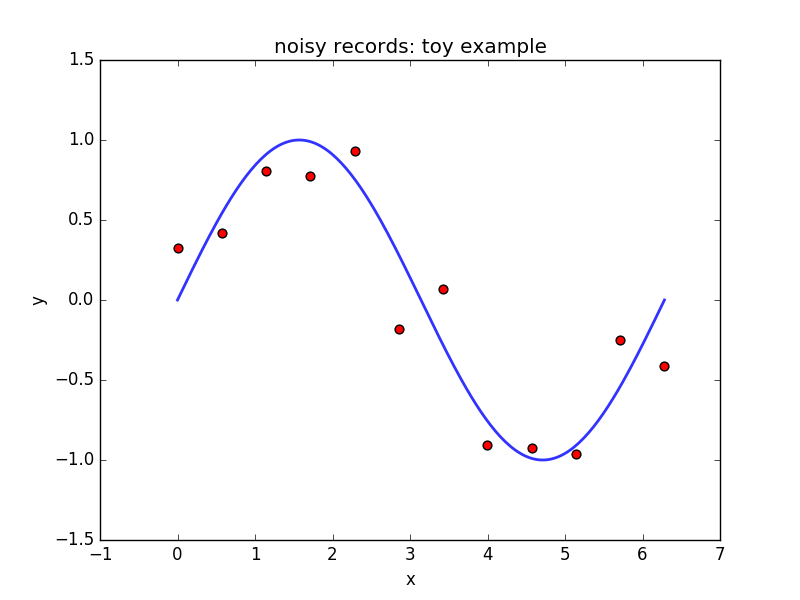
\includegraphics[width=0.6\textwidth]{../graphics/sample_from_sin.png}
\end{figure}
\begin{itemize}
	\item From a set of measured points $(x_i, y_i)$ (red), we would like to build a model to predict the value $y$ for any given $x$. 
	\item The true function is $g(x)=\sin (x)$ (displayed in blue).
	\item The measurements $y_i$ are noisy outputs of that function, i.e. 
	\begin{equation}
	y_i = \sin (x_i) + \epsilon \; , \;\;\; \;\;\; \epsilon \sim \mathcal{N}(0,0.2)
	\end{equation}
\end{itemize}
\end{frame}

\begin{frame}{A simple example: polynomial curve fitting}
\begin{figure}[htb]
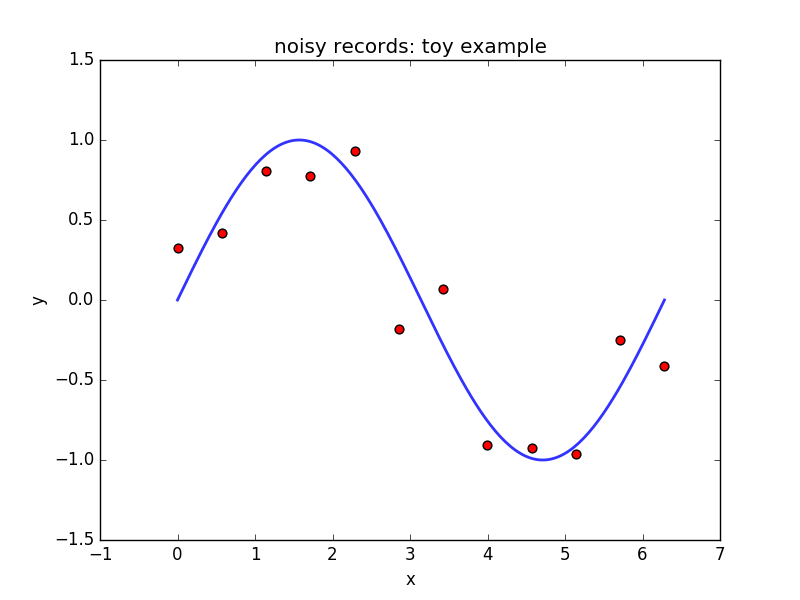
\includegraphics[width=0.6\textwidth]{../graphics/sample_from_sin.png}
\end{figure}
\begin{itemize}
	\item For this we use the following polynomial model:
	\begin{equation}
	f(x) = a_0 + a_1 x + a_2 x^2 + \ldots + a_m x^m
	\end{equation}
	\item The parameter vector is thus $\theta = (a_0, a_1, \ldots, a_m)^T$. 
	\item The model is linear in the parameters (but for $m>1$ not in the inputs). 
\end{itemize}
\end{frame}


%%%%%%%%%%%%%%%%%%%%%%%%%%%%%%%%%%%%%%%%%%%%%%%%%%%%%%%%%%%%%%%%%%%%%%%%%
%%%%%%%%%%%%%%%%%%%%%%%%%%%%%%%%%%%%%%%%%%%%%%%%%%%%%%%%%%%%%%%%%%%%%%%%%
\section{Supervised Learning: Example algorithms}
\subsection{Nearest Neighbor classification}
\subsection{Random Forests}
\subsection{Linear Discriminant Analysis (LDA)}
\subsection{Support Vector Machines (SVM) and kernel methods}


\end{document}